\documentclass[12pt]{article}
\usepackage{a4wide}
\usepackage{color, amssymb}
\usepackage[margin=1in]{geometry}
\usepackage[document]{ragged2e}
\usepackage[table]{xcolor}
\usepackage{multirow}
\usepackage[braket, qm]{qcircuit}
\setlength{\arrayrulewidth}{0.5mm}
\setlength{\tabcolsep}{16pt}
\renewcommand{\arraystretch}{1.9}
\usepackage[english,greek]{babel}
\usepackage{braket}
\usepackage{mathtools}
\usepackage{ragged2e}
\renewcommand{\baselinestretch}{1.5}
\input{epsf}
\usepackage{float}
\usepackage{graphicx}
\usepackage{caption}
\usepackage{subcaption}
\usepackage{algorithm}
\usepackage[noend]{algpseudocode}

\begin{document}

\greektext

\noindent\rule{\textwidth}{2pt}
\begin{center}
{\bf ΕΙΣΑΓΩΓΗ ΣΤΟΥΣ ΚΒΑΝΤΙΚΟΥΣ ΥΠΟΛΟΓΙΣΤΕΣ}\\ 
{\bf 2o Σετ Ασκήσεων }\\
{\bf Καλαμαράκης Θεόδωρος:} 2018030022\\
\end{center}
\rule{\textwidth}{.5pt}
\noindent

\begin{center}

\end{center}
 
 

\justifying

\section*{{\bf Μέρος  $\bf 1^o$ }}
\section*{Απο βιβλίο \textlatin{McMahon}}
\rule{\textwidth}{.5pt}
%%%%%%%%%%%%%%%%%%%%%%%%%%%%%%%%%%%%%%%%%%%%%%%%%%%%%%%%%%%%%%%%%%%%%%%%%%%%%%%%%%%%%%%%%%%%%%%%%%%%%%%%%%%%%%%%%%%%%%%%%%%%%%%%%%%%%%%
\section*{{\bfΆσκηση 4.1}}
Τα δαινύσαμτα βάσης είναι τα 
$$\ket{w_1}=\ket{0}  \otimes \ket{0}\;,\; \ket{w_2}=\ket{0}  \otimes \ket{0}\;,\; \ket{w_3}=\ket{1}  \otimes \ket{0}\;,\; \ket{w_4}=\ket{1}  \otimes \ket{1}$$
Αρχικά δείχνουμε οτι κάθε διάνυσμα είναι κανονικοποιημένο 
$$\braket{w_1|w_1} = \bra{0}\otimes \bra{0} \ket{0}\otimes\ket{1}=  \braket{0|0}\braket{0|0} = 1\cdot1=1$$
$$\braket{w_2|w_2} = \bra{0}\otimes \bra{1} \ket{0}\otimes\ket{1}=  \braket{0|0}\braket{1|1} = 1\cdot1=1$$
$$\braket{w_3|w_3} = \bra{1}\otimes \bra{0} \ket{1}\otimes\ket{0}=  \braket{1|1}\braket{0|0} = 1\cdot1=1$$
$$\braket{w_4|w_4} = \bra{1}\otimes \bra{1} \ket{1}\otimes\ket{1}=  \braket{1|1}\braket{1|1} = 1\cdot1=1$$\\
Για να είναι ορθοκανονικά τα διανύσαμτα βάσης πρέπει ανα δύο να έχουν εσωτερικό γινόμενο ίσο με 0.
$$\braket{w_1|w_2} = \bra{0}\otimes \bra{0} \ket{0}\otimes\ket{1}=  \braket{0|0}\braket{0|1} = 0\cdot1=0$$
$$\braket{w_1|w_3} = \bra{0}\otimes \bra{0} \ket{1}\otimes\ket{0}=  \braket{0|1}\braket{0|0} = 1\cdot0=0$$
$$\braket{w_1|w_4} = \bra{0}\otimes \bra{0} \ket{1}\otimes\ket{1}=  \braket{0|1}\braket{0|1} = 0\cdot0=0$$
$$\braket{w_2|w_3} = \bra{0}\otimes \bra{1} \ket{1}\otimes\ket{0}=  \braket{1|0}\braket{0|1} = 0\cdot0=0$$
$$\braket{w_2|w_4} = \bra{0}\otimes \bra{1} \ket{1}\otimes\ket{1}=  \braket{0|1}\braket{1|1} = 0\cdot1=0$$
$$\braket{w_3|w_4} = \bra{1}\otimes \bra{0} \ket{1}\otimes\ket{1}=  \braket{1|1}\braket{0|1} = 1\cdot0=0$$\\
Άρα είναι ορθοκανονικά.\\
\\ \rule{\textwidth}{.5pt}
%%%%%%%%%%%%%%%%%%%%%%%%%%%%%%%%%%%%%%%%%%%%%%%%%%%%%%%%%%%%%%%%%%%%%%%%%%%%%%%%%%%%%%%%%%%%%%%%%%%%%%%%%%%%%%%%%%%%%%%%%%%%%%%%%%%%%%%
\section*{{\bfΆσκηση 4.3}}
$$\braket{\psi|\phi} = (\bra{a}\otimes\bra{c})(\ket{b}\otimes\ket{d}) = \braket{a|b}\braket{c|d}=\frac{1}{2}\cdot\frac{3}{4}=\frac{3}{8} $$
 \\ \rule{\textwidth}{.5pt}
 %%%%%%%%%%%%%%%%%%%%%%%%%%%%%%%%%%%%%%%%%%%%%%%%%%%%%%%%%%%%%%%%%%%%%%%%%%%%%%%%%%%%%%%%%%%%%%%%%%%%%%%%%%%%%%%%%%%%%%%%%%%%%%%%%%%%%%%%
\section*{{\bfΆσκηση 4.4}}
{\centering
$ \ket{\psi} = \frac{1}{\sqrt{2}}\begin{pmatrix} 1\\ 1\end{pmatrix}$ και $ \ket{\phi} = \frac{1}{2}\begin{pmatrix} 1\\ \sqrt{3}\end{pmatrix}$
$$\ket{\psi}\otimes\ket{\phi} = \frac{1}{2\sqrt{2}}\begin{pmatrix}1\\\sqrt{3}\\1\\\sqrt{3}\end{pmatrix} $$
}
\rule{\textwidth}{.5pt}
%%%%%%%%%%%%%%%%%%%%%%%%%%%%%%%%%%%%%%%%%%%%%%%%%%%%%%%%%%%%%%%%%%%%%%%%%%%%%%%%%%%%%%%%%%%%%%%%%%%%%%%%%%%%%%%%%%%%%%%%%%%%%%%%%%%%%%%%%
\section*{{\bfΆσκηση 4.5}}
$$\ket{\psi} = \frac{1}{2}(\ket{0}\ket{0} - \ket{0}\ket{1} - \ket{1}\ket{0} + \ket{1}\ket{1})  = \ket{0}\otimes(\ket{0}-\ket{1})-ket{1}\otimes(\ket{0}-\ket{1}) =(\ket{0} - \ket{1})\otimes(\ket{0} - \ket{1})  $$

Συνεπώς μπορεί να γραφεί ώς γινόμενο κταστάσεων.\\
\rule{\textwidth}{.5pt}
%%%%%%%%%%%%%%%%%%%%%%%%%%%%%%%%%%%%%%%%%%%%%%%%%%%%%%%%%%%%%%%%%%%%%%%%%%%%%%%%%%%%%%%%%%%%%%%%%%%%%%%%%%%%%%%%%%%%%%%%%%%%%%%%%%%%%%%%%%
\section*{{\bfΆσκηση 4.6}}

$$\ket{\psi} = \frac{\ket{0}\ket{0} + \ket{1}\ket{1}}{\sqrt{2}} $$
Η παραπάνω κατάσταση αποτελεί μια απο τις καταστάσεις \textlatin{Bell} οι οποίες δεν είναι διαχωρίσιμες.
\rule{\textwidth}{.5pt}
%%%%%%%%%%%%%%%%%%%%%%%%%%%%%%%%%%%%%%%%%%%%%%%%%%%%%%%%%%%%%%%%%%%%%%%%%%%%%%%%%%%%%%%%%%%%%%%%%%%%%%%%%%%%%%%%%%%%%%%%%%%%%%%%%%%%%%%
\section*{{\bfΆσκηση 4.7}}
    Γνωρίζουμε οτι $X\ket{0}= \ket{1}$, $X\ket{1}= \ket{0}$, $Y\ket{0}= i\ket{1}$ και $Y\ket{1}= -i\ket{0}$\\
Άρα 
$$ X \otimes Y\ket{\psi} = X \otimes Y(\frac{\ket{0}\ket{1} - \ket{1}\ket{0}}{\sqrt{2}}) = \frac{(X\ket{0})\otimes(Y\ket{1}) - (X\ket{1})\otimes(Y\ket{0})}{\sqrt{2}}=$$ 
$$ = \frac{-i\ket{1}\ket{0} - i\ket{0}\ket{1}}{\sqrt{2}}=-\frac{i}{\sqrt{2}}(\ket{1}\ket{0} +\ket{0}\ket{1})$$\\
\rule{\textwidth}{.5pt}
\section*{{\bfΆσκηση 4.8}}
$$(A\otimes B)^\dag = \begin{pmatrix}\begin{bmatrix}
    a_{11}B & a_{12}B & ... & a_{1n}B \\
    a_{21}B & a_{22}B & ... & a_{2n}B \\
    \vdots &\vdots & \ddots& \vdots \\
    a_{m1}B & a_{m2}B & ... & a_{mn}B \\
\end{bmatrix}\end{pmatrix} ^\dag = \begin{bmatrix}
    a_{11}^*B^\dag &  a_{21}^*B^\dag & ... &  a_{m1}^*B^\dag \\
    a_{12}^*B^\dag & a_{22}^*B^\dag & ... &  a_{m2}^*B^\dag \\
    \vdots &\vdots & \ddots& \vdots \\
    a_{1n}^*B^\dag &  a_{2n}^*B^\dag & ... &  a_{mn}^*B^\dag \\
\end{bmatrix}= $$
$$=\begin{bmatrix}
    a_{11}^* &  a_{21}^* & ... &  a_{m1}^* \\
    a_{12}^* & a_{22}^* & ... &  a_{m2}^* \\
    \vdots &\vdots & \ddots& \vdots \\
    a_{1n}^* &  a_{2n}^* & ... &  a_{mn}^* \\
\end{bmatrix}\otimes B^\dag = A^\dag \otimes B^\dag$$
\\\rule{\textwidth}{.5pt}
%%%%%%%%%%%%%%%%%%%%%%%%%%%%%%%%%%%%%%%%%%%%%%%%%%%%%%%%%%%%%%%%%%%%%%%%%%%%%%%%%%%%%%%%%%%%%%%%%%%%%%%%%%%%%%%%%%%%%%%%%%%%%%%%%%%%%%
\section*{{\bfΆσκηση 4.9}}
    Γνωρίζουμε οτι $I\ket{0}= \ket{0}$, $I\ket{1}= \ket{1}$, $Y\ket{0}= i\ket{1}$ και $Y\ket{1}= -i\ket{0}$\\
Άρα 
$$ I \otimes Y\ket{\psi} = I \otimes Y(\frac{\ket{0}\ket{0} + \ket{1}\ket{1}}{\sqrt{2}}) = \frac{(I\ket{0})\otimes(Y\ket{0}) + (I\ket{1})\otimes(Y\ket{1})}{\sqrt{2}}=$$ 
$$ = \frac{i\ket{0}\ket{1} - i\ket{1}\ket{0}}{\sqrt{2}}=\frac{i}{\sqrt{2}}(\ket{0}\ket{1} -\ket{1}\ket{0})$$
\\\rule{\textwidth}{.5pt}
%%%%%%%%%%%%%%%%%%%%%%%%%%%%%%%%%%%%%%%%%%%%%%%%%%%%%%%%%%%%%%%%%%%%%%%%%%%%%%%%%%%%%%%%%%%%%%%%%%%%%%%%%%%%%%%%%%%%%%%%%%%%%%%%%%%%%
\section*{{\bfΆσκηση 4.10}}
{\centering
$X =\begin{bmatrix}
    0 & 1 \\ 
    1 & 0
\end{bmatrix} $ και $Y =\begin{bmatrix}
    0 & -i \\ 
    i & 0
\end{bmatrix} $\\
}
Αρα
$$ X \otimes Y = \begin{bmatrix}
    0Y & 1Y \\ 
    1Y & 0Y
\end{bmatrix}=\begin{bmatrix}
    0 & 0 & 0 & -i\\ 
    0 & 0 & i & 0 \\ 
    0 & -i& 0 & 0 \\ 
    i & 0 & 0 & 0
\end{bmatrix}$$
\\\rule{\textwidth}{.5pt}
%%%%%%%%%%%%%%%%%%%%%%%%%%%%%%%%%%%%%%%%%%%%%%%%%%%%%%%%%%%%%%%%%%%%%%%%%%%%%%%%%%%%%%%%%%%%%%%%%%%%%%%%%%%%%%%%%%%%%%%%%%%%%%%%%
\section*{{\bfΆσκηση 6.1}}
Για ναδείξουμε οτι είναι ο $P_1P_2$ είναι προβολικός τελεστής αρκεί να δείξουμε οτι:
{\centering
$P_1P_2=(P_1P_2)^\dag $ και $P_1P_2=(P_1P_2)^2 $
}
Εφόσον $P_1$ και $P_1$ είναι προβολικοί τελεστές γνωρίζουμε οτι $P_1^\dag = P_1$, $P_2^\dag = P_2$, $P_1^2 = P_1$, $P_2^2 = P_2$ και 
επιπλέον $[P_1,P_2]=0 \Leftrightarrow P_1P_2=P_2P_1$ 
Συνεπώς μπορούμε να πούμε οτι
 $$ (P_1P_2)^\dag = P_2^\dag P_1^\dag=P_2P_1=P_1P_2$$
 $$ (P_1P_2)^2 =(P_1P_2)(P_1P_2)= P_1(P_2P_1)P_2=P_1P_1P_2P_2=P_1^2P_2^2=P_1P_2$$
 Αρα είναι πράγματι προβολικός τελεστής
\\\rule{\textwidth}{.5pt}
%%%%%%%%%%%%%%%%%%%%%%%%%%%%%%%%%%%%%%%%%%%%%%%%%%%%%%%%%%%%%%%%%%%%%%%%%%%%%%%%%%%%%%%%%%%%%%%%%%%%%%%%%%%%%%%%%%%%%%%%%%%%%%%%%%%
\section*{{\bfΆσκηση 6.2}}
Aρχικά πρέπει να ελέγξουμε αν το σύστημα είναι κανονικοποιημένο υπολογίζοντας την ποσότητα
$$ \sum_{i=1}^{3}|c_i|^2 = (\frac{1}{2})^2+ (\frac{\sqrt{2}}{2})^2 + (\frac{1}{2})^2 = \frac{1}{4}+\frac{1}{2}+\frac{1}{4}=1$$
Που σημαίνει οτι είναι κανονικοποιημένο.\\ \\
Οι τρείς προβολικοί τελεστές είναι οι 
$$ P_1=\ket{u_1}\bra{u_1}$$
$$ P_2=\ket{u_2}\bra{u_2}$$
$$ P_3=\ket{u_3}\bra{u_3}$$

Οι αντίστοιχες πιθανότητες μέτρησης της της κάθε κατάστασης είναι 
$$Pr(u_1) = \braket{\psi|P_1|\psi} = | \braket{u_1|\psi}|^2 = | \frac{1}{2}\braket{u_1|u_1} -\frac{\sqrt{2}}{2}\braket{u_1|u_2}+\frac{1}{2}\braket{u_1|u_3}|^2$$
$$| \frac{1}{2}\cdot 1 -\frac{\sqrt{2}}{2}\cdot 0+\frac{1}{2}\cdot 0|^2 = | \frac{1}{2}|^2= \frac{1}{4}   $$
$$Pr(u_2) = \braket{\psi|P_2|\psi} = | \braket{u_2|\psi}|^2 = | \frac{1}{2}\braket{u_2|u_1} -\frac{\sqrt{2}}{2}\braket{u_2|u_2}+\frac{1}{2}\braket{u_2|u_3}|^2$$
$$| \frac{1}{2}\cdot 0 -\frac{\sqrt{2}}{2}\cdot 1+\frac{1}{2}\cdot 0|^2 = | -\frac{\sqrt{2}}{2}|^2= \frac{1}{2}   $$
$$Pr(u_3) = \braket{\psi|P_3|\psi} = | \braket{u_3|\psi}|^2 = | \frac{1}{2}\braket{u_3|u_1} -\frac{\sqrt{2}}{2}\braket{u_3|u_2}+\frac{1}{2}\braket{u_3|u_3}|^2$$
$$| \frac{1}{2}\cdot 0 -\frac{\sqrt{2}}{2}\cdot 0+\frac{1}{2}\cdot 1|^2 = | \frac{1}{2}|^2= \frac{1}{4}   $$
Η μέση ενέργεια του συστήματος υπολογίζεται απο τον τύπο $ \braket{H} = \sum_ih_i\braket{\psi|P_i|\psi}$. Άρα
$$\braket{H}=\hbar \omega \frac{1}{4} + 2\hbar \omega \frac{1}{2}+3\hbar \omega \frac{1}{4}=2\hbar \omega$$\\
\rule{\textwidth}{.5pt}
%%%%%%%%%%%%%%%%%%%%%%%%%%%%%%%%%%%%%%%%%%%%%%%%%%%%%%%%%%%%%%%%%%%%%%%%%%%%%%%%%%%%%%%%%%%%%%%%%%%%%%%%%%%%%%%%%%%%%%%%%




\section*{{\bfΆσκηση 6.3}}
Στην 1η σειρά ασκήσεων είχε αποδειχθεί οτι οι ιδιοτιμές του πίνακα $X$ είναι οι $\lambda_1=1$ και $\lambda _2=-1$ ενώ τα αντίστοιχα κανονικοποιήμένα διανύσαμτα είναι
$v_1=\frac{1}{\sqrt{2}}(\;1\;,\;1\;)^T$ και $v_2=\frac{1}{\sqrt{2}}(\;1\;,\;-1\;)^T$ αντίστοιχα.

Αρα για την ιδιοτιμή $\lambda_1$ ο προβολικός τελεστής είναι ο 
$$ P_1 = \ket{v_1}\bra{v_1} = \frac{1}{2}\begin{pmatrix}
    1\\1
\end{pmatrix}(\;1\;\;\;1\;) = \frac{1}{2}\begin{pmatrix}
    1&1\\1&1
\end{pmatrix}$$

ενω για την ιδιοτιμή $\lambda_2$ ο προβολικός τελεστής είναι ο
$$ P_2 = \ket{v_2}\bra{v_2} = \frac{1}{2}\begin{pmatrix}
    1\\-1
\end{pmatrix}(\;1\;\;\;-1\;) = \frac{1}{2}\begin{pmatrix}
    1&-1\\-1&1
\end{pmatrix}$$\\
Για να υπολογίσουμε τις πιθανότητες μέτρησης για κάθε μια απο τις δυο ιδιοτιμές ,θα χρησιμοποιήσουμε τον τύπο
$$Pr_i = \bra{\psi}P_i\ket{\psi} $$ \\
Αρχικά υπολογίζουμε 
$$ P_1\ket{\psi} = \frac{1}{2} \begin{pmatrix}
    1&1\\1&1
\end{pmatrix}\begin{pmatrix}
    0\\1
\end{pmatrix} = \frac{1}{2}\begin{pmatrix}
    1\\1
\end{pmatrix} $$

$$ P_2\ket{\psi} = \frac{1}{2} \begin{pmatrix}
    1&-1\\-1&1
\end{pmatrix}\begin{pmatrix}
    0\\1
\end{pmatrix} = \frac{1}{2}\begin{pmatrix}
    -1\\1
\end{pmatrix} $$

Αρα 
$$Pr(1) = \bra{\psi}P_1\ket{\psi} = \bra{1}\frac{1}{2}\begin{pmatrix}
    1\\1
\end{pmatrix} = \frac{1}{2}(\;0\;\;\;1\;)\begin{pmatrix}
    1\\1
\end{pmatrix}  =  \frac{1}{2}$$
$$Pr(-1) = \bra{\psi}P_2\ket{\psi} = \bra{1}\frac{1}{2}\begin{pmatrix}
    -1\\1
\end{pmatrix} = \frac{1}{2}(\;0\;\;\;1\;)\begin{pmatrix}
    -1\\1
\end{pmatrix}  =  \frac{1}{2}$$
\\\rule{\textwidth}{.5pt}
%%%%%%%%%%%%%%%%%%%%%%%%%%%%%%%%%%%%%%%%%%%%%%%%%%%%%%%%%%%%%%%%%%%%%%%%%%%%%%%%%%%%%%%%%%%%%%%%%%%%%%%%%%%%%%%%%%%%%%%%%
\section*{{\bfΆσκηση 6.4}}
$$\ket{\psi} = \frac{1}{\sqrt{3}}\ket{00}+\frac{1}{\sqrt{6}}\ket{01}+\frac{1}{\sqrt{2}}\ket{11}$$
{\bf (A)}\\
$$Pr(\ket{01}) = |\braket{01|\psi}|^2 = |\frac{1}{\sqrt{3}}\braket{01|00}+\frac{1}{\sqrt{6}}\braket{01|01}+\frac{1}{\sqrt{2}}\braket{01|11}|^2 = \
|\frac{1}{\sqrt{6}}|^2 = \frac{1}{6}$$\\
{\bf (B)}\\
Για να υπολογίσουμε την ζητούμενη πιθανότητα θα χρησιμοποιήσουμε τον τελεστή $I\otimes P_{\ket{1}} = I\otimes \ket{1}\bra{1}$\\
$$Pr = \braket{\psi|I\otimes \ket{1}\bra{1}|\psi} = \bra{\psi}(\frac{1}{\sqrt{3}}\ket{0}\otimes\ket{1}\braket{1|0}+\frac{1}{\sqrt{6}}\ket{0}\otimes\ket{1}\braket{1|1}+\frac{1}{\sqrt{2}}\ket{1}\otimes\ket{1}\braket{1|1})=$$
$$=\bra{\psi}(\frac{1}{\sqrt{6}}\ket{01}+\frac{1}{\sqrt{2}}\ket{11}) = (\frac{1}{\sqrt{3}}\bra{00}+\frac{1}{\sqrt{6}}\bra{01}+\frac{1}{\sqrt{2}}\bra{11})(\frac{1}{\sqrt{6}}\ket{01}+\frac{1}{\sqrt{2}}\ket{11}) =$$
$$= (\frac{1}{\sqrt{6}})^2 + (\frac{1}{\sqrt{2}})^2 = \frac{2}{3}$$\\
Η κατάσταση του συστήματος μετα την μέτρηση θα είναι 
$$\ket{\psi'} = \frac{I\otimes \ket{1}\bra{1}\ket{\psi} }{\sqrt{\braket{\psi|I\otimes \ket{1}\bra{1}|\psi}}}= 
\sqrt{\frac{3}{2}}(\frac{1}{\sqrt{6}}\ket{01}+\frac{1}{\sqrt{2}}\ket{11}) = \frac{1}{2}\ket{01}+\frac{\sqrt{3}}{2}\ket{11}$$\\
\rule{\textwidth}{.5pt}
%%%%%%%%%%%%%%%%%%%%%%%%%%%%%%%%%%%%%%%%%%%%%%%%%%%%%%%%%%%%%%%%%%%%%%%%%%%%%%%%%%%%%%%%%%%%%%%%%%%%%%%%%%%%%%%%%%%%%%%%%%%%
\section*{{\bfΆσκηση 6.5}}
Αρχικά θέλουμε να γράψουμε την κατάσταση $\ket{\psi}$ ως διάνυσμα στήλης (έχουμε ελέγξει οτι είναι κανονικοποιημένη λέγοντας $(\frac{1}{\sqrt{6}})^2 + (\frac{\sqrt{5}}{\sqrt{6}})^2 = \frac{1}{6} + \frac{5}{6}=1$)
$$\ket{\psi} = \frac{1}{\sqrt{6}}\ket{0}+\frac{\sqrt{5}}{\sqrt{6}}\ket{1} = \frac{1}{\sqrt{6}}\begin{pmatrix}1\\0\end{pmatrix}+\frac{\sqrt{5}}{\sqrt{6}}\begin{pmatrix}0\\1\end{pmatrix}=
 \frac{1}{\sqrt{6}}\begin{pmatrix}1\\\sqrt{5}\end{pmatrix}$$
 Στην 1η σειρά ασκήσεων είχε αποδειχθεί οτι οι ιδιοτιμές του πίνακα $Y$ είναι οι $\lambda_1=1$ και $\lambda_2=-1$ ενώ τα αντίστοιχα κανονικοποιημένα διανύσαμτα είναι
$v_1=\frac{1}{\sqrt{2}}(\;1\;,\;i\;)^T$ και $v_2=\frac{1}{\sqrt{2}}(\;1\;,\;-i\;)^T$ αντίστοιχα.

Για την ιδιοτιμή $\lambda_1$ ο προβολικός τελεστής είναι ο 
$$ P_1 = \ket{v_1}\bra{v_1} = \frac{1}{2}\begin{pmatrix}
    1\\i
\end{pmatrix}(\;1\;\;\;-i\;) = \frac{1}{2}\begin{pmatrix}
    1&-i\\i&1
\end{pmatrix}$$

ενω για την ιδιοτιμή $\lambda_2$ ο προβολικός τελεστής είναι ο
$$ P_2 = \ket{v_2}\bra{v_2} = \frac{1}{2}\begin{pmatrix}
    1\\-i
\end{pmatrix}(\;1\;\;\;i\;) = \frac{1}{2}\begin{pmatrix}
    1&i\\-i&1
\end{pmatrix}$$\\
Η μέση τιμή του$Y$ ως προς το $\ket{\psi}$ υπολογίζεται απο τον τύπο 
$$ \braket{X} = \sum_i \lambda_i\braket{\psi|P_i|\psi} = \lambda_1\braket{\psi|P_1|\psi} + \lambda_2\braket{\psi|P_2|\psi}=$$
$$= \frac{1}{\sqrt{6}}(\;1\;\;\;\sqrt{5}\;)\frac{1}{2}\begin{pmatrix}
    1&-i\\i&1
\end{pmatrix}\frac{1}{\sqrt{6}}\begin{pmatrix}1\\\sqrt{5}\end{pmatrix} - \frac{1}{\sqrt{6}}(\;1\;\;\;\sqrt{5}\;)\frac{1}{2}\begin{pmatrix}
    1&i\\-i&1
\end{pmatrix}\frac{1}{\sqrt{6}}\begin{pmatrix}1\\\sqrt{5}\end{pmatrix} =$$
$$=\frac{1}{12}(\;1\;\;\;\sqrt{5}\;)\begin{pmatrix}1-\sqrt{5}i\\i+\sqrt{5}\end{pmatrix} - 
\frac{1}{12}(\;1\;\;\;\sqrt{5}\;)\begin{pmatrix}1+\sqrt{5}i\\-i+\sqrt{5}\end{pmatrix} = $$
$$= \frac{1}{12}(1 - \sqrt{5}i+\sqrt{5}i+5 -(1 + \sqrt{5}i-\sqrt{5}i+5) ) = 0$$
\rule{\textwidth}{.5pt}
%%%%%%%%%%%%%%%%%%%%%%%%%%%%%%%%%%%%%%%%%%%%%%%%%%%%%%%%%%%%%%%%%%%%%%%%%%%%%%%%%%%%%%%%%%%%%%%%%%%%%%%%%%%%%%%%%%%%%%%%%%%%%
\section*{{\bfΆσκηση 6.6}}
$$\ket{\psi} = (\frac{\sqrt{2}+i}{\sqrt{20}})\ket{000}+\frac{1}{\sqrt{2}}\ket{001} + \frac{1}{\sqrt{10}}\ket{011}+\frac{i}{2}\ket{111}$$
Ελεγχουμε οτι το σύστημα είναι κανονικοποιημένο λέγοντας οτι
$$ |\frac{\sqrt{2}+i}{\sqrt{20}}|^2+|\frac{1}{\sqrt{2}}|^2+|\frac{1}{\sqrt{10}}|^2+|\frac{i}{2}|^2 = \frac{3}{20}+\frac{1}{2}+\frac{1}{10}+\frac{1}{4}=1$$\\
{\bf { (\textlatin{A})}}
$$Pr(\ket{011})= |\braket{011|\psi}|^2=\bra{011}((\frac{\sqrt{2}+i}{\sqrt{20}})\ket{000}+\frac{1}{\sqrt{2}}\ket{001} + \frac{1}{\sqrt{10}}\ket{011}+\frac{i}{2}\ket{111})=$$
$$ =  |(\frac{\sqrt{2}+i}{\sqrt{20}})\braket{011|000}+\frac{1}{\sqrt{2}}\braket{011|001} + \frac{1}{\sqrt{10}}\braket{011|011}+\frac{i}{2}\braket{011|111}|^2=|\frac{1}{\sqrt{10}}|^2=\frac{1}{10}$$\\
{\bf { (\textlatin{B})}}\\
Για το υπολογισμό της ζητούμενη πιθανότητας θα χρησιμοποιήσουμετον τελεστή $ P= I\otimes\ket{1}\bra{1}\otimes I$
$$Pr = \braket{\psi|P|\psi} = \bra{\psi}(I\otimes\ket{1}\bra{1}\otimes I((\frac{\sqrt{2}+i}{\sqrt{20}})\ket{000}+\frac{1}{\sqrt{2}}\ket{001} + \frac{1}{\sqrt{10}}\ket{011}+\frac{i}{2}\ket{111}))$$
$$=\bra{\psi}((\frac{\sqrt{2}+i}{\sqrt{20}})\ket{0}(\ket{1}\braket{1|0})\ket{0}+\frac{1}{\sqrt{2}}\ket{0}(\ket{1}\braket{1|0})\ket{1} + \frac{1}{\sqrt{10}}\ket{0}(\ket{1}\braket{1|1})\ket{1}+\frac{i}{2}\ket{1}(\ket{1}\braket{1|1})\ket{1})$$
$$=\bra{\psi}(\frac{1}{\sqrt{10}}\ket{011}+\frac{i}{2}\ket{111})=((\frac{\sqrt{2}+i}{\sqrt{20}})\bra{000}+\frac{1}{\sqrt{2}}\bra{001} + \frac{1}{\sqrt{10}}\bra{011}+\frac{i}{2}\bra{111})(\frac{1}{\sqrt{10}}\ket{011}+\frac{i}{2}\ket{111})$$
$$=|\frac{1}{\sqrt{10}}|^2+|\frac{i}{2}|^2 = \frac{1}{10}+\frac{1}{4}=\frac{7}{20}$$
Η κατάσταση μετά την μέτρηση υπολογίζεται ώς εξής:
$$\ket{\psi} = \frac{P\ket{\psi}}{\sqrt{\braket{\psi|P|\psi}}} = \sqrt{\frac{20}{7}}(\frac{1}{\sqrt{10}}\ket{011}+\frac{i}{2}\ket{111})=\sqrt{\frac{2}{7}}\ket{011}+\sqrt{\frac{5}{7}}i\ket{111})$$\\
Η κατάσταση που προέκυψε είναι κανονικοποιημένη καθώς 
$$ |\sqrt{\frac{2}{7}}|^2 + |\sqrt{\frac{5}{7}}ι|^2 = \frac{2}{7} +\frac{5}{7}=1$$\\
\rule{\textwidth}{.5pt}
%%%%%%%%%%%%%%%%%%%%%%%%%%%%%%%%%%%%%%%%%%%%%%%%%%%%%%%%%%%%%%%%%%%%%%%%%%%%%%%%%%%%%%%%%%%%%%%%%%%%%%%%%%%%%%%%%%%%%%%%%%%%%
\section*{{\bfΆσκηση 6.7}}
$$\ket{\phi} = \frac{1}{\sqrt{6}}\ket{01}+\sqrt{\frac{5}{6}}\ket{10}$$
Ελεγχουμε αρχικά αν το σύστημα είναι κανονικοποιημένο υπολογίζοντας την ποσότητα
$$ \sum_{i=1}^{3}|c_i|^2 = (\frac{1}{\sqrt{6}})^2+ (\sqrt{\frac{5}{6}})^2=\frac{1}{6} +\frac{5}{6} =1$$
Αρα είναι κανονικοποιημένη\\
Έπειτα εφαρμόζουμε τον τελεστή $P= I \otimes X$ στην $\ket{\phi}$ ωστε η πύλη $X$ να δράσει μόνο στο δεύτερο \textlatin{qubit} και έχουμε:
$$P\ket{\phi} = I \otimes X(\frac{1}{\sqrt{6}}\ket{01}+\sqrt{\frac{5}{6}}\ket{10}) = \frac{1}{\sqrt{6}}\ket{0}X\ket{1}+\sqrt{\frac{5}{6}}\ket{1}X\ket{0}=$$
$$=\frac{1}{\sqrt{6}}\ket{00}+\sqrt{\frac{5}{6}}\ket{11}$$\\
Παρατηρούμε οτι στην νέα κατάσταση τα μόνα πιθανά αποτελέσματα μέτρησης είναι τα $00$ και $11$. Για κάθε ένα απο αυτά η πιθανότητα μέτρησης είναι:
$$Pr(00) = |\bra{00}P\ket{\phi}|^2 = |\bra{00}(\frac{1}{\sqrt{6}}\ket{00}+\sqrt{\frac{5}{6}}\ket{11})|^2 
= |\frac{1}{\sqrt{6}}\braket{00|00}+\sqrt{\frac{5}{6}}\braket{00|11}|^2 = \frac{1}{6}$$ 
$$Pr(11) = |\bra{11}P\ket{\phi}|^2 = |\bra{11}(\frac{1}{\sqrt{6}}\ket{00}+\sqrt{\frac{5}{6}}\ket{11})|^2 
= |\frac{1}{\sqrt{6}}\braket{11|00}+\sqrt{\frac{5}{6}}\braket{11|11}|^2 = \frac{5}{6}$$ \
\rule{\textwidth}{.5pt}
%%%%%%%%%%%%%%%%%%%%%%%%%%%%%%%%%%%%%%%%%%%%%%%%%%%%%%%%%%%%%%%%%%%%%%%%%%%%%%%%%%%%%%%%%%%%%%%%%%%%%%%%%%%%%%%%%%%%%%%%%%%%%
\section*{{\bfΆσκηση 7.1 }}

Έστω οτι τα $\ket{+_n} , \ket{-_n}$ είναι όντως τα ιδιοδιανύσαματα του $\vec{\sigma}\cdot \vec{n}$. Τότε θα ισχύει
$$\vec{\sigma}\cdot \vec{n} =\ket{+_n}\bra{+_n} - \ket{-_n}\bra{-_n}  = \begin{pmatrix}\cos^2\frac{\theta}{2} & e^{-i\phi}\cos{\frac{\theta}{2}}\sin{\frac{\theta}{2}} \\ e^{i\phi}\cos{\frac{\theta}{2}}\sin{\frac{\theta}{2}} &\sin^2\frac{\theta}{2} \end{pmatrix} 
- \begin{pmatrix}\sin^2\frac{\theta}{2} & -e^{-i\phi}\cos{\frac{\theta}{2}}\sin{\frac{\theta}{2}} \\ -e^{i\phi}\cos{\frac{\theta}{2}}\sin{\frac{\theta}{2}} &\cos^2\frac{\theta}{2} \end{pmatrix}  = $$ 
$$ =  \begin{pmatrix}\cos^2\frac{\theta}{2} - \sin^2\frac{\theta}{2} & 2e^{-i\phi}\cos{\frac{\theta}{2}}\sin{\frac{\theta}{2}} \\ 2e^{i\phi}\cos{\frac{\theta}{2}}\sin{\frac{\theta}{2}} &\sin^2\frac{\theta}{2}-\cos^2\frac{\theta}{2} \end{pmatrix} $$
Γνωρίζουμε οτι 

$$ \cos^2\frac{\theta}{2} - \sin^2\frac{\theta}{2} = \cos\theta$$
$$ 2\cos{\frac{\theta}{2}}\sin{\frac{\theta}{2}} = \sin\theta $$

Ara 
$$\vec{\sigma}\cdot \vec{n} =  \begin{pmatrix}\cos\theta & \cos\phi \sin\theta - i \sin\phi \sin\theta \\ \cos\phi \sin\theta + i \sin\phi \sin\theta &-\cos\theta \end{pmatrix} =$$
$$ \cos\theta \begin{pmatrix}
    1&0\\0&-1
\end{pmatrix} + \cos\phi \sin\theta \begin{pmatrix}
    0&1\\1&0
\end{pmatrix} + \sin\phi \sin\theta \begin{pmatrix}
    0&-i\\i&0
\end{pmatrix} = $$
$$\cos\theta Z + \cos\phi\sin\theta X + \sin\theta\sin\theta Y$$\\
\rule{\textwidth}{.5pt}
%%%%%%%%%%%%%%%%%%%%%%%%%%%%%%%%%%%%%%%%%%%%%%%%%%%%%%%%%%%%%%%%%%%%%%%%%%%%%%%%%%%%%%%%%%%%%%%%%%%%%%%%%%%%%%%%%%%%%%%%%%%%%
\section*{{\bfΆσκηση 7.2}}
$$ \ket{\psi} = \frac{\ket{0}\ket{1} - \ket{1}\ket{0}}{\sqrt{2}}$$

Τα ιδιοδιανύσματα του τελεστή $Y$ είναι τα 
$$\ket{\pm _y} = \frac{\ket{0} \pm \ket{1}}{\sqrt{2}}$$ 
Θέλουμε να βρούμε το $\ket{0}$ και $\ket{1}$ συναρτήσει τών ιδιοδιανύσματων $\ket{\pm _y}$ 
$$\ket{+_y} + \ket{-_y} = \frac{\ket{0} + i\ket{1}+\ket{0} - i\ket{1}}{\sqrt{2}}  = \frac{2\ket{0}}{\sqrt{2}} \Leftrightarrow \ket{0} = \frac{\ket{+_y} + \ket{-_y}}{\sqrt{2}} $$
$$\ket{+_y} - \ket{-_y} = \frac{\ket{0} + i\ket{1}-\ket{0} + i\ket{1}}{\sqrt{2}}  = \frac{2i\ket{1}}{\sqrt{2}} \Leftrightarrow \ket{1} = \frac{-i\ket{+_y} +i\ket{-_y}}{\sqrt{2}} $$

Ξαναγράφουμε την κατάσταση $\ket{\psi}$
$$\ket{\psi} = \frac{\ket{0}\ket{1} - \ket{1}\ket{0}}{\sqrt{2}} =  \frac{\frac{\ket{+_y} + \ket{-_y}}{\sqrt{2}}\frac{-i\ket{+_y} +i\ket{-_y}}{\sqrt{2}} - \frac{-i\ket{+_y} +i\ket{-_y}}{\sqrt{2}}\frac{\ket{+_y} + \ket{-_y}}{\sqrt{2}}}{\sqrt{2}}$$
$$  =  \frac{(\ket{+_y} + \ket{-_y})(-i\ket{+_y} +i\ket{-_y})-(-i\ket{+_y} +i\ket{-_y})(\ket{+_y} + \ket{-_y})}{2\sqrt{2}} = $$
$$ = \frac{-i\ket{+_y+_y} + i\ket{+_y-_y}-i\ket{-_y+_y} + i\ket{-_y-_y}+i\ket{+_y+_y} +i\ket{+_y-_y}-i\ket{-_y+_y} + -i\ket{-_y-_y}}{2\sqrt{2}}=$$
$$ = \frac{2i\ket{+_y-_y}-2i\ket{-_y+_y} }{2\sqrt{2}}= \frac{i\ket{+_y-_y}-i\ket{-_y+_y} }{\sqrt{2}}$$
Η οποία στην ουσία είνιαι η ίδια κατάσταση αφου αν μετρήσουμε την κατάσταση του πρώτου \textlatin{qubit} να είναι $\ket{+_y}$ 
τότε αναγκαστικά η κατάσταση του δεύτερου θα είναι $\ket{-_y}$ ενώ αν μετρήσουμε την κατάσταση του πρώτου να είναι $\ket{-_y}$
τότε αναγκαστικά η κατάσταση του δεύτερου θα είναι $\ket{+_y}$. Ίδια ακριβώς συμπεριφορά (δηλαδή το ένα να είναι το ανάποδο του άλλου) παρατηρείται και αν κάνουμε την μέτρηση στο άξονα $Z$\\
\rule{\textwidth}{.5pt}
%%%%%%%%%%%%%%%%%%%%%%%%%%%%%%%%%%%%%%%%%%%%%%%%%%%%%%%%%%%%%%%%%%%%%%%%%%%%%%%%%%%%%%%%%%%%%%%%%%%%%%%%%%%%%%%%%%%%%%%%%%%%%
\section*{{\bfΆσκηση 7.3}}
Γνωρίζουμε οτι η δράση του  τελεστή $Z$ είναι $Z\ket{0} = \ket{0} $ και $Z\ket{1} = \ket{1}$. Αρα
$$Z\otimes Z\ket{\beta_{00}} =  Z\otimes Z\frac{\ket{00} +\ket{11}}{\sqrt{2}} =\frac{Z\ket{0}\otimes Z\ket{0} +Z\ket{1}\otimes Z\ket{1}}{\sqrt{2}} 
=\frac{\ket{00} + \ket{11}}{\sqrt{2}}$$
Επίσης
$$(-1)^y\ket{\beta_{xy}} \Big|_{x=0,y=0} = \ket{\beta_{00}}= \frac{\ket{00} + \ket{11}}{\sqrt{2}}$$
Αρα βλέπουμε οτι πράγματι $Z\otimes Z\ket{\beta_{xy}}=(-1)^y\ket{\beta_{xy}}$ για $x=0,y=0$\\
Αντιστοιχα 

$$Z\otimes Z\ket{\beta_{01}} =  Z\otimes Z\frac{\ket{01} +\ket{10}}{\sqrt{2}} =\frac{Z\ket{0}\otimes Z\ket{1} +Z\ket{1}\otimes Z\ket{0}}{\sqrt{2}} 
=-\frac{\ket{01} + \ket{10}}{\sqrt{2}}$$
Επίσης
$$(-1)^y\ket{\beta_{xy}} \Big|_{x=0,y=1} = -\ket{\beta_{01}}= -\frac{\ket{01} + \ket{10}}{\sqrt{2}}$$
Αρα βλέπουμε οτι πράγματι $Z\otimes Z\ket{\beta_{xy}}=(-1)^y\ket{\beta_{xy}}$ για $x=0,y=0$\\
\rule{\textwidth}{.5pt}
%%%%%%%%%%%%%%%%%%%%%%%%%%%%%%%%%%%%%%%%%%%%%%%%%%%%%%%%%%%%%%%%%%%%%%%%%%%%%%%%%%%%%%%%%%%%%%%%%%%%%%%%%%%%%%%%%%%%%%%%%%%%%
\section*{{\bfΆσκηση 7.4}}
Γνωρίζουμε οτι η δράση του  τελεστή $X$ είναι $X\ket{y} = \ket{\overline{y}} $. Αρα
$$X\otimes X\ket{\beta_{xy}} =  X\otimes X\frac{\ket{0y} +(-1)^x\ket{1\overline{y}}}{\sqrt{2}} =\frac{X\ket{0}\otimes X\ket{y} +(-1)^xX\ket{1}\otimes X\ket{\overline{y}}}{\sqrt{2}} 
=\frac{\ket{1\overline{y}} +(-1)^x\ket{0y}}{\sqrt{2}}$$
βγάζοντας το $(-1)^x$ κοινό παράγοντα έχουμε:
$$X\otimes X\ket{\beta_{xy}} = (-1)^x\frac{(-1)^{-x}\ket{1\overline{y}} +\ket{0y}}{\sqrt{2}}=(-1)^x\frac{(\frac{1}{-1})^{x}\ket{1\overline{y}} +\ket{0y}}{\sqrt{2}}=$$
$$=(-1)^x\frac{(-1)^{x}\ket{1\overline{y}} +\ket{0y}}{\sqrt{2}} = (-1)^x\ket{\beta_{xy}}$$\\
\rule{\textwidth}{.5pt}
%%%%%%%%%%%%%%%%%%%%%%%%%%%%%%%%%%%%%%%%%%%%%%%%%%%%%%%%%%%%%%%%%%%%%%%%%%%%%%%%%%%%%%%%%%%%%%%%%%%%%%%%%%%%%%%%%%%%%%%%%%%%%
\section*{{\bfΆσκηση 7.5}}
Γνωρίζουμε οτι η δράση του  τελεστή $Y$ είναι $Y\ket{x} = (-1)^xi\ket{\overline{x}} $. Αρα
$$Y\otimes Y\ket{\beta_{xy}} =  Y\otimes Y\frac{\ket{0y} +(-1)^x\ket{1\overline{y}}}{\sqrt{2}} =\frac{Y\ket{0}\otimes Y\ket{y} +(-1)^xY\ket{1}\otimes Y\ket{\overline{y}}}{\sqrt{2}} =$$
$$=\frac{i\ket{1}(-1)^yi\ket{\overline{y}} +(-i)\ket{0}(-1)^x(-1)^{\overline{y}}i\ket{y}}{\sqrt{2}}
=\frac{-(-1)^y\ket{1\overline{y}} +(-1)^x(-1)^{\overline{y}}\ket{0y}}{\sqrt{2}}$$
Παρατηρούμε οτι $(-1)^{\overline{y}} = -(-1)^y $ Ara
$$Y\otimes Y\ket{\beta_{xy}} = \frac{-(-1)^y\ket{1\overline{y}} -(-1)^x(-1)^{y}\ket{0y}}{\sqrt{2}}=-(-1)^y\frac{\ket{1\overline{y}} +(-1)^x\ket{0y}}{\sqrt{2}} =$$
$$=-(-1)^y(-1)^x\frac{(-1)^{-x}\ket{1\overline{y}} +\ket{0y}}{\sqrt{2}} =- (-1)^{y+x}\frac{(-1)^{x}\ket{1\overline{y}} +\ket{0y}}{\sqrt{2}}= - (-1)^{y+x}\ket{\beta_{xy}}$$\\
\rule{\textwidth}{.5pt}
%%%%%%%%%%%%%%%%%%%%%%%%%%%%%%%%%%%%%%%%%%%%%%%%%%%%%%%%%%%%%%%%%%%%%%%%%%%%%%%%%%%%%%%%%%%%%%%%%%%%%%%%%%%%%%%%%%%%%%%%%%%%%
\section*{{\bfΆσκηση 7.6}}
Αρχικά παρατηρούμε οτι 
$$ XZ = \begin{pmatrix*}
    0 & 1 \\ 1 & 0
\end{pmatrix*}\begin{pmatrix*}
    1 & 0 \\ 0 & -1
\end{pmatrix*}   = \begin{pmatrix*}
    0 & -1 \\ 1 & 0
\end{pmatrix*} $$και
$$ ZX = \begin{pmatrix*}
    1 & 0 \\ 0 & -1
\end{pmatrix*} \begin{pmatrix*}
    0 & 1 \\ 1 & 0
\end{pmatrix*}  = \begin{pmatrix*}
    0 & 1 \\ -1 & 0
\end{pmatrix*} = -XZ \;\;(1)$$

Γνωρίζοντας αυτό μπορούμε να γράψουμε οτι:
$$[X\otimes X,Z\otimes Z] =(X\otimes X)(Z\otimes Z )- (Z\otimes Z)(X\otimes X) = XZ\otimes XZ - ZX\otimes ZX \xLeftrightarrow{(1)} $$
$$[X\otimes X,Z\otimes Z] = XZ\otimes XZ - (-XZ)\otimes (-XZ) =XZ\otimes XZ - XZ\otimes XZ = 0 $$
\rule{\textwidth}{.5pt}
%%%%%%%%%%%%%%%%%%%%%%%%%%%%%%%%%%%%%%%%%%%%%%%%%%%%%%%%%%%%%%%%%%%%%%%%%%%%%%%%%%%%%%%%%%%%%%%%%%%%%%%%%%%%%%%%%%%%%%%%%%%%%

\section*{{\bfΆσκηση 7.7}}

\begin{itemize}
\item $$
        \vec{\sigma_A}\cdot\vec{\sigma_A}\ket{\phi_1} = \begin{pmatrix*}
            1 &0& 0& 0\\
            0 &-1 &2& 0 \\ 
            0 &2& -1 &0 \\ 
            0 &0 &0 &1
        \end{pmatrix*} \frac{1}{\sqrt{2}}\begin{pmatrix*}
            0\\1\\1\\0
        \end{pmatrix*} = \frac{1}{\sqrt{2}}\begin{pmatrix*}
            0\\1\\1\\0
        \end{pmatrix*} = \ket{\phi_1}
        $$
\item  $$
        \vec{\sigma_A}\cdot\vec{\sigma_A}\ket{\phi_2} = \begin{pmatrix*}
            1 &0& 0& 0\\
            0 &-1 &2& 0 \\ 
            0 &2& -1 &0 \\ 
            0 &0 &0 &1
        \end{pmatrix*} \begin{pmatrix*}
            0\\0\\0\\1
        \end{pmatrix*} =\begin{pmatrix*}
            0\\0\\0\\1
        \end{pmatrix*} = \ket{\phi_2}
        $$
 \item  $$
        \vec{\sigma_A}\cdot\vec{\sigma_A}\ket{\phi_3} = \begin{pmatrix*}
            1 &0& 0& 0\\
            0 &-1 &2& 0 \\ 
            0 &2& -1 &0 \\ 
            0 &0 &0 &1
        \end{pmatrix*} \begin{pmatrix*}
            1\\0\\0\\0
        \end{pmatrix*} =\begin{pmatrix*}
            1\\0\\0\\0
        \end{pmatrix*} = \ket{\phi_3}
        $$

\item  $$
        \vec{\sigma_A}\cdot\vec{\sigma_A}\ket{\phi_4} = \begin{pmatrix*}
            1 &0& 0& 0\\
            0 &-1 &2& 0 \\ 
            0 &2& -1 &0 \\ 
            0 &0 &0 &1
        \end{pmatrix*} \frac{1}{\sqrt{2}}\begin{pmatrix*}
            0\\1\\-1\\0
        \end{pmatrix*} =\frac{1}{\sqrt{2}}\begin{pmatrix*}
            0\\-3\\3\\0
        \end{pmatrix*} = -3\frac{1}{\sqrt{2}}\begin{pmatrix*}
            0\\1\\-1\\0
        \end{pmatrix*} = -3\ket{\phi_4}
        $$       
    \end{itemize}


    \rule{\textwidth}{.5pt}
    %%%%%%%%%%%%%%%%%%%%%%%%%%%%%%%%%%%%%%%%%%%%%%%%%%%%%%%%%%%%%%%%%%%%%%%%%%%%%%%%%%%%%%%%%%%%%%%%%%%%%%%%%%%%%%%%%%%%%%%%%%%%%
    
    \section*{{\bfΆσκηση 8.3}}   
    $$ X^{11} = \ket{0}\bra{0},\;\;\;\;X^{12} = \ket{0}\bra{1}$$
    $$ X^{21} = \ket{1}\bra{0},\;\;\;\;X^{22} = \ket{1}\bra{1}$$ 
\begin{itemize}
 \item Για τον πίνακα $X$:
        $$X= \ket{0}\bra{1} + \ket{1}\bra{0}= X^{12} + X^{21}$$

 \item Για τον πίνακα $Y$:
        $$Y= -i\ket{0}\bra{1} + i\ket{1}\bra{0}= -iX^{12} + iX^{21}$$
 \item Για τον πίνακα $Z$:
        $$Z= \ket{0}\bra{0}  -\ket{1}\bra{1}= X^{11}  - X^{22}$$             
\end{itemize}    
\rule{\textwidth}{.5pt}
%%%%%%%%%%%%%%%%%%%%%%%%%%%%%%%%%%%%%%%%%%%%%%%%%%%%%%%%%%%%%%%%%%%%%%%%%%%%%%%%%%%%%%%%%%%%%%%%%%%%%%%%%%%%%%%%%%%%%%%%%%%%%

\section*{{\bfΆσκηση 8.4}}  
Γνωρίζουμε οτι $$CN \begin{pmatrix*}
    1 &0& 0& 0\\
    0 &1 &2& 0 \\ 
    0 &2& 0 &1 \\ 
    0 &0 &1 &0
\end{pmatrix*} $$
Αρχικά δείχνουμε οτι είναι ερμιτιανός 
$$CN^\dag =    \begin{pmatrix*}
    1 &0& 0& 0\\
    0 &1 &0& 0 \\ 
    0 &0& 0 &1 \\ 
    0 &0 &1 &0
\end{pmatrix*}^\dag = \begin{pmatrix*}
    1 &0& 0& 0\\
    0 &1 &0& 0 \\ 
    0 &0& 0 &1 \\ 
    0 &0 &1 &0
\end{pmatrix*} = CN $$

 Έπειτα για να δείξουμε οτι είναι \textlatin{unitary} λέμε:
 $$CN ^\dag CN =    \begin{pmatrix*}
    1 &0& 0& 0\\
    0 &1 &0& 0 \\ 
    0 &0& 0 &1 \\ 
    0 &0 &1 &0
\end{pmatrix*}\begin{pmatrix*}
    1 &0& 0& 0\\
    0 &1 &0& 0 \\ 
    0 &0& 0 &1 \\ 
    0 &0 &1 &1
\end{pmatrix*} = \begin{pmatrix*}
    1 &0& 0& 0\\
    0 &1 &0& 0 \\ 
    0 &0& 1 &0 \\ 
    0 &0 &0 &1 
\end{pmatrix*} = Ι$$\\ \\
\rule{\textwidth}{.5pt}
%%%%%%%%%%%%%%%%%%%%%%%%%%%%%%%%%%%%%%%%%%%%%%%%%%%%%%%%%%%%%%%%%%%%%%%%%%%%%%%%%%%%%%%%%%%%%%%%%%%%%%%%%%%%%%%%%%%%%%%%%%%%%
\section*{{\bfΆσκηση 8.5}}  
Αρχικά για $\ket{b}= \ket{0}$ έχουμε $\ket{ab} = \ket{10}$ άρα η κατάσταση που θα προκύψει είναι η:
\begin{align*}
    \ket{\psi} &= CN\cdot H\otimes I \ket{10} =CN \ket{-0} = CN \frac{\ket{00} -  \ket{10}}{\sqrt{2}} =\frac{ CN \ket{00} -   CN \ket{10}}{\sqrt{2}} =\\
    &=\frac{\ket{00} -  \ket{11}}{\sqrt{2}} = \ket{\beta_{10}}
\end{align*}
Για $\ket{b}= \ket{1}$ έχουμε $\ket{ab} = \ket{11}$ άρα η κατάσταση που θα προκύψει είναι η:
\begin{align*}
    \ket{\psi} &= CN\cdot H\otimes I \ket{11} =CN \ket{-1} = CN \frac{\ket{01} -  \ket{11}}{\sqrt{2}} =\frac{ CN \ket{01} -   CN \ket{11}}{\sqrt{2}} =\\
    &=\frac{\ket{01} -  \ket{10}}{\sqrt{2}} = \ket{\beta_{11}}\\ \\
\end{align*}
\rule{\textwidth}{.5pt}
%%%%%%%%%%%%%%%%%%%%%%%%%%%%%%%%%%%%%%%%%%%%%%%%%%%%%%%%%%%%%%%%%%%%%%%%%%%%%%%%%%%%%%%%%%%%%%%%%%%%%%%%%%%%%%%%%%%%%%%%%%%%%

\section*{{\bfΆσκηση 8.6}} 
Γνωρίζοντας οτι η δράση της πύλης $Z$ είναι $Z\ket{0} = \ket{0}$ και $Z\ket{1} = -\ket{1}$
Η απεικόνιση σε πίνακα της πύλης $Z$ είναι $$Z = \begin{pmatrix*}
    \bra{0}Ζ\ket{0} &\bra{0}Ζ\ket{1}\\
    \bra{1}Ζ\ket{0} &\bra{1}Ζ\ket{1}  
\end{pmatrix*} =  \begin{pmatrix*}
    1 &0\\
    0 &-1
\end{pmatrix*}$$\\
Ενώ η απεικόνιση σε συμβολισμό \textlatin{Dirac} $$Z= \ket{0}\bra{0}  -\ket{1}\bra{1}$$ \\ 
\rule{\textwidth}{.5pt}
%%%%%%%%%%%%%%%%%%%%%%%%%%%%%%%%%%%%%%%%%%%%%%%%%%%%%%%%%%%%%%%%%%%%%%%%%%%%%%%%%%%%%%%%%%%%%%%%%%%%%%%%%%%%%%%%%%%%%%%%%%%%%

\section*{{\bfΆσκηση 8.7}} 

\begin{itemize}
    \item Για τον πίνακα $X$ $$X^2 =  \begin{pmatrix*}
        0 &1\\
        1 &0
    \end{pmatrix*} \begin{pmatrix*}
        0 &1\\
        1 &0
    \end{pmatrix*} =  \begin{pmatrix*}
        1 &0\\
        0 &1
    \end{pmatrix*}$$
    \item Για τον πίνακα $Y$ $$Y^2 =  \begin{pmatrix*}
        0 &-i\\
        i &0
    \end{pmatrix*} \begin{pmatrix*}
        0 &-i\\
        i &0
    \end{pmatrix*} =  \begin{pmatrix*}
        1 &0\\
        0 &1
    \end{pmatrix*}$$
    \item Για τον πίνακα $Z$ $$Z^2 =  \begin{pmatrix*}
        1 &0\\
        0 &-1
    \end{pmatrix*} \begin{pmatrix*}
        1 &0\\
        0 &-1
    \end{pmatrix*} =  \begin{pmatrix*}
        1 &0\\
        0 &1
    \end{pmatrix*}$$
    \item Για τον πίνακα $T$ $$T^2 =  \begin{pmatrix*}
        1 &0\\
        0 &e^{\frac{i\pi}{4}}
    \end{pmatrix*} \begin{pmatrix*}
        1 &0\\
        0 &e^{\frac{i\pi}{4}}
    \end{pmatrix*} =  \begin{pmatrix*}
        1 &0\\
        0 &e^{\frac{i\pi}{2}}
    \end{pmatrix*}$$
    \item Για τον πίνακα $S$ $$S^2 =  \begin{pmatrix*}
        1 &0\\
        0 &i
    \end{pmatrix*} \begin{pmatrix*}
        1 &0\\
        0 &i
    \end{pmatrix*} =  \begin{pmatrix*}
        1 &0\\
        0 &-i
    \end{pmatrix*}$$\\ \\

\end{itemize}
\rule{\textwidth}{.5pt}
%%%%%%%%%%%%%%%%%%%%%%%%%%%%%%%%%%%%%%%%%%%%%%%%%%%%%%%%%%%%%%%%%%%%%%%%%%%%%%%%%%%%%%%%%%%%%%%%%%%%%%%%%%%%%%%%%%%%%%%%%%%%%

\section*{{\bfΆσκηση 8.10}} 
Γνωρίζοντας οτι 
$$P_0\ket{0} = \ket{0}\bra{0}\ket{0} = \ket{0}$$
$$P_0\ket{1} = \ket{0}\bra{0}\ket{1} =0$$
$$P_1\ket{1} = \ket{1}\bra{1}\ket{1} = \ket{0}$$
$$P_1\ket{0} = \ket{1}\bra{1}\ket{0} =0$$ \\ 
Θα μελετήσουεμ την δράση του τελεστή $P_0\otimes I + P_1\otimes X$  εφαρμόζοντας τον σε κάθε μια απο τις δυνατές καταστάσεις των δύο \textlatin{qubit}
\begin{itemize}
    \item $$(P_0\otimes I + P_1\otimes X)\ket{00} = P_0\ket{0}\otimes I\ket{0} + P_1\ket{0}\otimes X\ket{0} = \ket{00}$$
    \item $$(P_0\otimes I + P_1\otimes X)\ket{01} = P_0\ket{0}\otimes I\ket{1} + P_1\ket{0}\otimes X\ket{1} = \ket{01}$$
    \item $$(P_0\otimes I + P_1\otimes X)\ket{10} = P_0\ket{1}\otimes I\ket{0} + P_1\ket{1}\otimes X\ket{0} = \ket{11}$$
    \item $$(P_0\otimes I + P_1\otimes X)\ket{11} = P_0\ket{1}\otimes I\ket{1} + P_1\ket{1}\otimes X\ket{1} = \ket{10}$$\\
\end{itemize}
Παρατηρούμε λοιπόν οτι η συμπεριφορά είναι ίδια με την συμπεριφορά της πύλης $CN$ άρα $CN = P_0\otimes I + P_1\otimes X$\\ \\
\rule{\textwidth}{.5pt}
%%%%%%%%%%%%%%%%%%%%%%%%%%%%%%%%%%%%%%%%%%%%%%%%%%%%%%%%%%%%%%%%%%%%%%%%%%%%%%%%%%%%%%%%%%%%%%%%%%%%%%%%%%%%%%%%%%%%%%%%%%%%%

\section*{{\bfΆσκηση 8.11}}

Παρατηρούμε οτι το πρώτο κύκλωμα είναι μια πύλη \textlatin{control NOT}  με το πρώτο \textlatin{qubit} να είναι το \textlatin{target} και το δεύτερο να είναι το\textlatin{control}
Συνεπώς ο τελεστής που το αντιπροσωπεύει είναι ο :
$$I\otimes P_0  + X\otimes P_1 = \begin{pmatrix*}
    1P_0 &0P_0\\
    0P_0 &1P_0
\end{pmatrix*} + \begin{pmatrix*}
    0P_1 &1P_1\\
    1P_1 &0P_1
\end{pmatrix*} = \begin{pmatrix*}
    1 &0 & 0& 0\\
    0 &0 & 0&0 \\
    0 &0 & 1& 0\\
    0 &0 & 0&0 \\
\end{pmatrix*} + \begin{pmatrix*}
    0 &0 & 0& 0\\
    0 &0 & 0&1 \\
    0 &0 & 0& 0\\
    0 &1 & 0&0 \\
\end{pmatrix*} = \begin{pmatrix*}
    1 &0 & 0& 0\\
    0 &0 & 0&1 \\
    0 &0 & 1& 0\\
    0 &1 & 0&0 \\
\end{pmatrix*}$$ \\ 
Ενώ για το δεύτερο κύκλωμα ο τελεστής είναι :
\begin{align*}
    (H\otimes H)(P_0\otimes I + P_1\otimes X)(H\otimes H) &=  \frac{1}{2}\begin{pmatrix*}
        1 &1 & 1& 1\\
        1 &-1 & 1&-1 \\
        1 &1 & -1& -1\\
        1 &-1 & -1&1 \\
    \end{pmatrix*}  \begin{pmatrix*}
        1 &0& 0& 0\\
        0 &1 &0& 0 \\ 
        0 &0& 0 &1 \\ 
        0 &0 &1 &0
    \end{pmatrix*}\frac{1}{2}\begin{pmatrix*}
        1 &1 & 1& 1\\
        1 &-1 & 1&-1 \\
        1 &1 & -1& -1\\
        1 &-1 & -1&1 \\
    \end{pmatrix*} = \\
    & = \frac{1}{4} \begin{pmatrix*}
    1 &1 & 1& 1\\
    1 &-1 & -1&1 \\
    1 &1 & -1& -1\\
    1 &-1 & 1&-1 \\
\end{pmatrix*}\begin{pmatrix*}
1 &1 & 1& 1\\
1 &-1 & 1&-1 \\
1 &1 & -1& -1\\
1 &-1 & -1&1 \\
\end{pmatrix*} = \\ 
&=\frac{1}{4}\begin{pmatrix*}
    4 &0 & 0& 0\\
    0 &0 & 0&4 \\
    0 &0 & 4& 0\\
    0 &4 & 0&0 \\
\end{pmatrix*} =\begin{pmatrix*}
    1 &0 & 0& 0\\
    0 &0 & 0&1 \\
    0 &0 & 1& 0\\
    0 &1 & 0&0 \\
\end{pmatrix*}\\
&= I\otimes P_0  + X\otimes P_1 \\
\end{align*}
 Άρα τα δύο κυκλώματα είναι όντως ισοδύναμα\\
 \rule{\textwidth}{.5pt}
 %%%%%%%%%%%%%%%%%%%%%%%%%%%%%%%%%%%%%%%%%%%%%%%%%%%%%%%%%%%%%%%%%%%%%%%%%%%%%%%%%%%%%%%%%%%%%%%%%%%%%%%%%%%%%%%%%%%%%%%%%%%%%
 
 \section*{{\bfΆσκηση 9.1}}

 $$H \otimes H = \frac{1}{\sqrt{2}} \begin{pmatrix*}
    1H &1H\\
    1H &-1H
\end{pmatrix*} =\frac{1}{2}\begin{pmatrix*}
    1 &1 & 1& 1\\
    1 &-1 & 1&-1 \\
    1 &1 & -1& -1\\
    1 &-1 & -1&1 \\
\end{pmatrix*}  $$ 
$$(H \otimes H ) (\ket{0}\otimes \ket{1})=\frac{1}{2}\begin{pmatrix*}
    1 &1 & 1& 1\\
    1 &-1 & 1&-1 \\
    1 &1 & -1& -1\\
    1 &-1 & -1&1 \\
\end{pmatrix*}  \begin{pmatrix*}
   0\\
   1\\
   0\\
   0\\
\end{pmatrix*} = \frac{1}{2}\begin{pmatrix*}
    1\\
    -1\\
    1\\
    -1\\
 \end{pmatrix*} $$ 
Eπιπλέον 
$$\ket{\phi}= \left(\frac{\ket{0}+\ket{1}}{\sqrt{2}}\right)\left(\frac{\ket{0}-\ket{1}}{\sqrt{2}}\right) = \frac{1}{2}\begin{pmatrix*}
    1\\
    1
 \end{pmatrix*}\otimes\begin{pmatrix*}
    1\\
    -1
 \end{pmatrix*}=\frac{1}{2}\begin{pmatrix*}
    1\\
    -1\\
    1\\
    -1
 \end{pmatrix*}$$

 Συνεπώς $(H \otimes H ) (\ket{0}\otimes \ket{1}) = \ket{\phi}$\\
 \rule{\textwidth}{.5pt}
 %%%%%%%%%%%%%%%%%%%%%%%%%%%%%%%%%%%%%%%%%%%%%%%%%%%%%%%%%%%%%%%%%%%%%%%%%%%%%%%%%%%%%%%%%%%%%%%%%%%%%%%%%%%%%%%%%%%%%%%%%%%%%
 
 \section*{{\bfΆσκηση 9.4}}
 Για την σχέση $(9.17)\;\;\;\ket{0,1\oplus f(0)}= f(0)\ket{00}  + (1-f(0))\ket{01}$ 
 \begin{itemize}
    \item Για $f(0) = 0\;\;\longrightarrow \ket{0,1\oplus 0} = 0\cdot\ket{00}  + (1-0)\ket{01} \Leftrightarrow \ket{01} = \ket{01}$   {\it Ισχύει}
    \item Για $f(0) = 1\;\;\longrightarrow \ket{0,1\oplus 1} = 1\cdot\ket{00}  + (1-1)\ket{01} \Leftrightarrow \ket{00} = \ket{00}$   {\it Ισχύει}
\end{itemize}
Για την σχέση $(9.18)\;\;\;\ket{1,0\oplus f(1)}= (1-f(1))\ket{10}  + f(1)\ket{11}$ 
 \begin{itemize}
    \item Για $f(1) = 0\;\;\longrightarrow \ket{1,0\oplus 0}= (1-0)\ket{10}  + 0\cdot \ket{11} \Leftrightarrow \ket{10} = \ket{10}$   {\it Ισχύει}
    \item Για $f(1) = 1\;\;\longrightarrow \ket{1,0\oplus 1} =(1-1)\ket{10}  + 1\cdot \ket{11} \Leftrightarrow \ket{11} = \ket{11}$   {\it Ισχύει}
\end{itemize}
Για την σχέση $(9.19)\;\;\;\ket{1,1\oplus f(1)}= f(1)\ket{10}+(1-f(1))\ket{11}  $ 
 \begin{itemize}
    \item Για $f(1) = 0\;\;\longrightarrow \ket{1,1\oplus 0}= 0\cdot\ket{10}  + (1-0)\ket{11} \Leftrightarrow \ket{11} = \ket{11}$   {\it Ισχύει}
    \item Για $f(1) = 1\;\;\longrightarrow \ket{1,1\oplus 1}= 1\cdot\ket{10}  + (1-1)\ket{11} \Leftrightarrow \ket{10} = \ket{10}$   {\it Ισχύει}\\
 \end{itemize}
 \rule{\textwidth}{.5pt}
 %%%%%%%%%%%%%%%%%%%%%%%%%%%%%%%%%%%%%%%%%%%%%%%%%%%%%%%%%%%%%%%%%%%%%%%%%%%%%%%%%%%%%%%%%%%%%%%%%%%%%%%%%%%%%%%%%%%%%%%%%%%%%
 
 \section*{{\bfΆσκηση 9.5}}
 Έστω οτι συμβολίζουμε με $Α$ τον αθροιστή μα ςκαι έστω οτι την πύλη $\ket{z}$ την έχουμε μόνιμα σε κατάσταση $\ket{0}$.\\ 
 Τότε τπ αποτέλεσμα που θέλουμε να πετύχουμε είναι το παρακάτω:
 $$A\ket{000} = \ket{000}$$
 $$A\ket{010} = \ket{010}$$
 $$A\ket{100} = \ket{110}$$
 $$A\ket{110} = \ket{101}$$\
 Tο αποτέλεσμα αυτο επιτυγχάνεται με το παρακάτω κύκλωμα


 \begin{figure}[H]
    
    \centering
    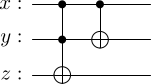
\includegraphics[scale=1]{adderrqiskit.png}\\
\end{figure}
H έξοδος $\ket{x\oplus y}$ υλοποιείται με μία απλή \textlatin{control NOT} με το $x$ να είναι το \textlatin{control} και το $y$ το \textlatin{target},
 ενώ η έξοδος $\ket{x\cdot y}$ υλοποιείται με μία διπλή \textlatin{control NOT} (\textlatin{Toffoli}) me \textlatin{control} ta $x$ kai $y$
 \rule{\textwidth}{.5pt}
 %%%%%%%%%%%%%%%%%%%%%%%%%%%%%%%%%%%%%%%%%%%%%%%%%%%%%%%%%%%%%%%%%%%%%%%%%%%%%%%%%%%%%%%%%%%%%%%%%%%%%%%%%%%%%%%%%%%%%%%%%%%%%

 \section*{{\bf Μέρος  $\bf 2^o$ }}
 \section*{{\bfΆσκηση 1}}
 \subsection*{{\bf Ερώτημα 1}}
 $$ \det |X-\lambda I| = 0 \Leftrightarrow \det \begin{vmatrix}\begin{pmatrix}\;0 \;\; & 1 \;\;\\ \;1 \;\; & 0 \;\;\end{pmatrix} -\begin{pmatrix}\;\lambda \;\; & 0 \;\;\\\;0 \;\; & \lambda \;\;\end{pmatrix}\end{vmatrix}  =0 \Leftrightarrow$$

$$ \Leftrightarrow\det \begin{vmatrix}\;-\lambda \;\; & 1 \;\;\\ \;1 \;\; & -\lambda \;\;\end{vmatrix} = \lambda^2 -1=0 $$ \\
Άρα οι ιδιοτιμές είναι οι $\lambda_1 = 1$ και $\lambda_2=-1$ \\
Για τα ιδιοδιανύσματα έχουμε:
Εστω $\ket{v}=\begin{pmatrix} v_1 \\ v_2\end{pmatrix}$
$$X\ket{v}=\lambda\ket{ v} \Leftrightarrow \begin{pmatrix}\;0 \;\; & 1 \;\;\\ \;1 \;\; & 0 \;\;\end{pmatrix}\begin{pmatrix} v_1 \\ v_2\end{pmatrix}=\lambda\begin{pmatrix} v_1 \\ v_2\end{pmatrix} \Leftrightarrow 
\begin{pmatrix} v_2 \\ v_1\end{pmatrix} = \lambda \begin{pmatrix} v_1 \\ v_2\end{pmatrix}$$\\
Για $\lambda =1 $ τότε $v_1=v_2$ άρα $\ket{v_1} = \frac{1}{\sqrt{2}}(\;1\;,\;1\;)^T = \ket{+}$ \\
Για $\lambda =-1 $ τότε $v_1=-v_2$ άρα $\ket{v_2} = \frac{1}{\sqrt{2}}(\;1\;,\;-1\;)^T= \ket{-}$\\ \\
\subsection*{{\bf Ερώτημα 2}}
Στο πρώτο κύκλωμα το αποτέλεσμα είναι το παρακάτω
\begin{center}
    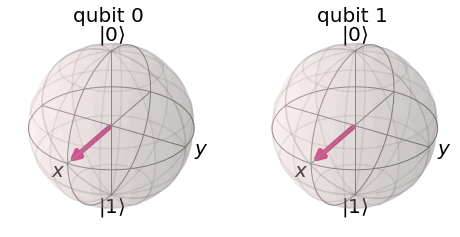
\includegraphics[]{notphasekickback.png}
\end{center}

Παρατηρούμε οτι δεν υπάρχει \textlatin{phase kickback} καθώς στη πρώτη είσοδο βάλαμε $\ket{0}$ και μετα την εφαρμογή της \textlatin{Hadamard} πήραμε το $\ket{+}$ όπως αναμενόταν \\ 
Στο δεύτερο κύκλωμα το αποτέλεσμα είναι 
\begin{center}
    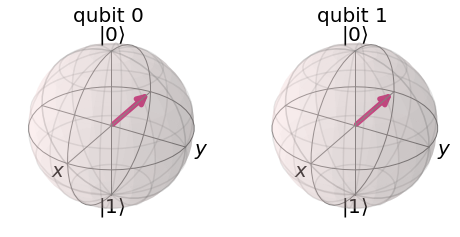
\includegraphics[]{phasekickback.png}
\end{center}


Παρατηρούμε οτι υπάρχει \textlatin{phase kickback} καθώς στη πρώτη είσοδο βάλαμε $\ket{0}$ και μετα την εφαρμογή της \textlatin{Hadamard} πήραμε το $\ket{-}$ , και ο λόγος είναι οτι αντίστρέψαμε την δεύτερη είσοδο (την κάναμε $\ket{1}$) πρίν εφαρμόσουμε την \textlatin{Hadamard}\\
\rule{\textwidth}{.5pt}

%%%%%%%%%%%%%%%%%%%%%%%%%%%%%%%%%%%%%%%%%%%%%%%%%%%%%%%%%%%%%%%%%%%%%%%%%%%%%%%%%%%%%%%%%%%%%%%%%%%%%%%%%%%%%%%%%%%%%%%%%%%%%

\section*{{\bfΆσκηση 2}}
Για το πρώτο κύκλωμα 
$$
(X\cdot T \cdot T  \cdot Z  \cdot S \cdot H \cdot Z \cdot H) \otimes ( \cdot Z \cdot Y \cdot X) = $$
$$=\begin{pmatrix} 0 & 1 \\ 1 & 0\end{pmatrix}\begin{pmatrix} 1 & 0 \\ 0 & e^{\frac{i\pi}{4}}\end{pmatrix}\begin{pmatrix} 1 & 0 \\ 0 & e^{\frac{i\pi}{4}}\end{pmatrix}
\begin{pmatrix} 1 & 0 \\ 0 & -1\end{pmatrix}\begin{pmatrix} 1 & 0 \\ 0 & i\end{pmatrix}\frac{1}{\sqrt{2}}\begin{pmatrix} 1 & 1\\ 1 &-1\end{pmatrix}\begin{pmatrix} 1 & 0 \\ 0 & -1\end{pmatrix}
\frac{1}{\sqrt{2}}\begin{pmatrix} 1 & 1\\ 1 &-1\end{pmatrix}$$
$$ \otimes \begin{pmatrix} 1 & 0 \\ 0 & -1 \end{pmatrix}\begin{pmatrix} 0 & -i \\ i & 0\end{pmatrix}\begin{pmatrix} 0 & 1 \\ 1 & 0\end{pmatrix}  = 
$$
$$=\begin{pmatrix} 0 & e^{\frac{i\pi}{4}}\\ 1 &0 \end{pmatrix}\begin{pmatrix} 1 & 0 \\ 0 & e^{\frac{i\pi}{4}}\end{pmatrix}
\begin{pmatrix} 1 & 0 \\ 0 & -1\end{pmatrix}\begin{pmatrix} 1 & 0 \\ 0 & i\end{pmatrix}\frac{1}{\sqrt{2}}\begin{pmatrix} 1 & 1\\ 1 &-1\end{pmatrix}\begin{pmatrix} 1 & 0 \\ 0 & -1\end{pmatrix}
\frac{1}{\sqrt{2}}\begin{pmatrix} 1 & 1\\ 1 &-1\end{pmatrix}$$
$$ \otimes\begin{pmatrix} 0 & -i \\ -i & 0 \end{pmatrix}\begin{pmatrix} 0 & 1 \\ 1 & 0\end{pmatrix}  = 
$$

$$=\begin{pmatrix} 0 & i \\ 1 & 0 \end{pmatrix} \begin{pmatrix} 1 & 0 \\ 0 & -1\end{pmatrix}\begin{pmatrix} 1 & 0 \\ 0 & i\end{pmatrix}\frac{1}{\sqrt{2}}\begin{pmatrix} 1 & 1\\ 1 &-1\end{pmatrix}\begin{pmatrix} 1 & 0 \\ 0 & -1\end{pmatrix}
\frac{1}{\sqrt{2}}\begin{pmatrix} 1 & 1\\ 1 &-1\end{pmatrix}$$
$$ \otimes\begin{pmatrix} -i & 0 \\ 0& -i\end{pmatrix}  = 
$$
$$=\begin{pmatrix} 0 & -i\\ 1 & 0\end{pmatrix}\begin{pmatrix} 1 & 0 \\ 0 & i\end{pmatrix}\frac{1}{\sqrt{2}}\begin{pmatrix} 1 & 1\\ 1 &-1\end{pmatrix}\begin{pmatrix} 1 & 0 \\ 0 & -1\end{pmatrix}
\frac{1}{\sqrt{2}}\begin{pmatrix} 1 & 1\\ 1 &-1\end{pmatrix}
 \otimes\begin{pmatrix} -i & 0 \\ 0& -i\end{pmatrix}  = 
$$
$$=\left(\begin{pmatrix} 0 & 1 \\ 1 & 0\end{pmatrix}\frac{1}{\sqrt{2}}\begin{pmatrix} 1 & 1\\ 1 &-1\end{pmatrix}\begin{pmatrix} 1 & 0 \\ 0 & -1\end{pmatrix}
\frac{1}{\sqrt{2}}\begin{pmatrix} 1 & 1\\ 1 &-1\end{pmatrix}\right)
 \otimes\begin{pmatrix} -i & 0 \\ 0& -i\end{pmatrix}  = 
$$
$$=\frac{1}{2}\left(\begin{pmatrix} 1 & -1\\ 1 &1\end{pmatrix}\begin{pmatrix} 1 & 0 \\ 0 & -1\end{pmatrix}
\begin{pmatrix} 1 & 1\\ 1 &-1\end{pmatrix}\right)
 \otimes\begin{pmatrix} -i & 0 \\ 0& -i\end{pmatrix}  = 
$$
$$=\frac{1}{2}\left(\begin{pmatrix} 1 & 1 \\ 1 & -1\end{pmatrix}
\begin{pmatrix} 1 & 1\\ 1 &-1\end{pmatrix}\right)
 \otimes\begin{pmatrix} -i & 0 \\ 0& -i\end{pmatrix}  = 
$$
$$=\frac{1}{2}\begin{pmatrix} 2 & 0 \\ 0 & 2\end{pmatrix}
 \otimes\begin{pmatrix} -i & 0 \\ 0& -i\end{pmatrix}  = 
$$
$$ \begin{pmatrix} 
    -i&0&0&0\\
    0&-i&0&0\\
    0&0&-i&0\\ 
    0&0&0&-i


\end{pmatrix}$$
Προσομοιώνοντας το κύκλωμα στο \textlatin{qiskit}
το αποτέλεσμα ήταν το ίδιο
\begin{center}
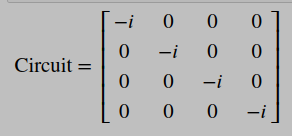
\includegraphics[]{2022-11-30_03-01.png}
\end{center}
Για το δεύτερο κύκλωμα 
$$R_Y(\frac{\pi}{2}) = \begin{pmatrix}
    \cos(\frac{\pi}{4}) &  -\sin(\frac{\pi}{4}) \\
    \sin(\frac{\pi}{4}) &  \cos(\frac{\pi}{4})
\end{pmatrix} = \begin{pmatrix}
    \frac{\sqrt{2}}{2} &  -\frac{\sqrt{2}}{2}\\
    \frac{\sqrt{2}}{2} & \frac{\sqrt{2}}{2}
\end{pmatrix} $$
Για την \textlatin{control} $R_Y(\frac{\pi}{2})$ (με αντιστραμμένο \textlatin{target} και \textlatin{{control}}) κάνουμε
\begin{align*}
    I \otimes P_0  + R_Y(\frac{\pi}{2}) \otimes P_1  &=  \begin{pmatrix}
        1 & 0\\
        0 & 1
    \end{pmatrix}\otimes\begin{pmatrix}
        1 & 0\\
        0 & 0
    \end{pmatrix} + \begin{pmatrix}
        \frac{\sqrt{2}}{2} &  -\frac{\sqrt{2}}{2}\\
        \frac{\sqrt{2}}{2} & \frac{\sqrt{2}}{2}
    \end{pmatrix} \otimes\begin{pmatrix}
        0 & 0\\
        0 & 1
    \end{pmatrix}=\\
    &= \begin{pmatrix}
        1 & 0 & 0&0\\
        0 & 0 & 0& 0\\
        0 & 0 & 1&0\\
        0 & 0 & 0& 0
    \end{pmatrix} + \begin{pmatrix}
        0 & 0 & 0&0\\
        0 & \frac{\sqrt{2}}{2} & 0& -\frac{\sqrt{2}}{2}\\
        0 & 0 & 0  & 0\\
        0 & \frac{\sqrt{2}}{2} & 0 & \frac{\sqrt{2}}{2}
    \end{pmatrix} = \begin{pmatrix}
        1 & 0 & 0&0\\
        0 & \frac{\sqrt{2}}{2} & 0& -\frac{\sqrt{2}}{2}\\
        0 & 0 & 1  & 0\\
        0 & \frac{\sqrt{2}}{2} & 0 & \frac{\sqrt{2}}{2}
    \end{pmatrix}
\end{align*}

Για την \textlatin{control} $H$ (με αντιστραμμένο \textlatin{target} και \textlatin{{control}})κάνουμε
\begin{align*}
    I \otimes P_0 + H\otimes P_1  &=  \begin{pmatrix}
        1 & 0\\
        0 & 1
    \end{pmatrix}\otimes\begin{pmatrix}
        1 & 0\\
        0 & 0
    \end{pmatrix} + \frac{1}{\sqrt{2}}\begin{pmatrix}
        1 & 1\\
        1 & -1
    \end{pmatrix}\otimes\begin{pmatrix}
        0 & 0\\
        0 & 1
    \end{pmatrix} =\\
    &= \begin{pmatrix}
        1 & 0 & 0&0\\
        0 & 0 & 0& 0\\
        0 & 0 & 1&0\\
        0 & 0 & 0& 0
    \end{pmatrix} + \frac{1}{\sqrt{2}}\begin{pmatrix}
        0 & 0 & 0&0\\
        0 & 1 & 0& 1\\
        0 & 0 & 0 & 0\\
        0 & 1 & 0 & -1
    \end{pmatrix} = \begin{pmatrix}
        1 & 0 & 0&0\\
        0 & \frac{1}{\sqrt{2}} & 0& \frac{1}{\sqrt{2}}\\
        0 & 0 & 1& 0\\
        0 & \frac{1}{\sqrt{2}} & 0& -\frac{1}{\sqrt{2}}
    \end{pmatrix} 
\end{align*}

Για την \textlatin{control} $X$  κάνουμε
\begin{align*}
    P_0 \otimes I + P_1 \otimes X &=  \begin{pmatrix}
        1 & 0\\
        0 & 0
    \end{pmatrix}\otimes\begin{pmatrix}
        1 & 0\\
        0 & 1
    \end{pmatrix} + \begin{pmatrix}
        0 & 0\\
        0 & 1
    \end{pmatrix}\otimes\begin{pmatrix}
        0 &  1\\
        1 & 0
    \end{pmatrix} =\\
    &= \begin{pmatrix}
        1 & 0 & 0&0\\
        0 & 1 & 0& 0\\
        0 & 0 & 0&0\\
        0 & 0 & 0& 0
    \end{pmatrix} + \begin{pmatrix}
        0 & 0 & 0&0\\
        0 & 0 & 0& 0\\
        0 & 0 &  & 1\\
        0 & 0 & 1 & 0
    \end{pmatrix} = \begin{pmatrix}
        1 & 0 & 0&0\\
        0 & 1 & 0& 0\\
        0 & 0 & 0& 1\\
        0 & 0 & 1& 0
    \end{pmatrix} 
\end{align*}

Αρα για το συνολικό κύκλωμα έχουμε

$$C R_Y(\frac{\pi}{2})\cdot C H \cdot (I \otimes Η)\cdot CX \cdot (I \otimes Η) = $$
$$=\begin{pmatrix}
    1 & 0 & 0&0\\
    0 & \frac{\sqrt{2}}{2} & 0& -\frac{\sqrt{2}}{2}\\
    0 & 0 & 1  & 0\\
    0 & \frac{\sqrt{2}}{2} & 0 & \frac{\sqrt{2}}{2}
\end{pmatrix}\begin{pmatrix}
    1 & 0 & 0&0\\
    0 & \frac{1}{\sqrt{2}} & 0& \frac{1}{\sqrt{2}}\\
    0 & 0 & 1& 0\\
    0 & \frac{1}{\sqrt{2}} & 0& -\frac{1}{\sqrt{2}}
\end{pmatrix}  \frac{1}{\sqrt{2}}\begin{pmatrix}
    1 & 1 & 0&0\\
    1 & -1 & 0& 0\\
    0 & 0 & 1& 1\\
    0 & 0 & 1& -1
\end{pmatrix}
\begin{pmatrix}
    1 & 0 & 0&0\\
    0 & 1 & 0& 0\\
    0 & 0 & 0& 1\\
    0 & 0 & 1& 0
\end{pmatrix} 
\frac{1}{\sqrt{2}}\begin{pmatrix}
    1 & 1 & 0&0\\
    1 & -1 & 0& 0\\
    0 & 0 & 1& 1\\
    0 & 0 & 1& -1
\end{pmatrix}
 = 
 $$
 $$\frac{1}{2}\begin{pmatrix}
    2 & 0 & 0&0\\
    0 & 2 & 0& 0\\
    0 & 0 & 2& 0\\
    0 & 0 & 0& 2
\end{pmatrix}
 = \begin{pmatrix}
    1 & 0 & 0&0\\
    0 & 1 & 0& 0\\
    0 & 0 & 1& 0\\
    0 & 0 & 0& 1
\end{pmatrix}$$

Προσομοιώνοντας το κύκλωμα στο \textlatin{qiskit}
το αποτέλεσμα ήταν το ίδιο
\begin{center}
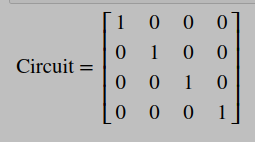
\includegraphics[]{2022-11-30_03-02.png}
\end{center}

\rule{\textwidth}{.5pt}

%%%%%%%%%%%%%%%%%%%%%%%%%%%%%%%%%%%%%%%%%%%%%%%%%%%%%%%%%%%%%%%%%%%%%%%%%%%%%%%%%%%%%%%%%%%%%%%%%%%%%%%%%%%%%%%%%%%%%%%%%%%%%

\section*{{\bfΆσκηση 4}} 

Για την \textlatin{constant} συνάρτηση έχουμε επιλέξει το \textlatin{oracle} $I \otimes I$ όπως φαίνεται παρακάτω
\begin{center}
    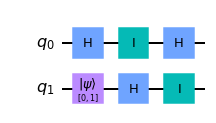
\includegraphics[]{constantoracle.png}
    \end{center}
το αποτέλεσμα είναι
\begin{center}
    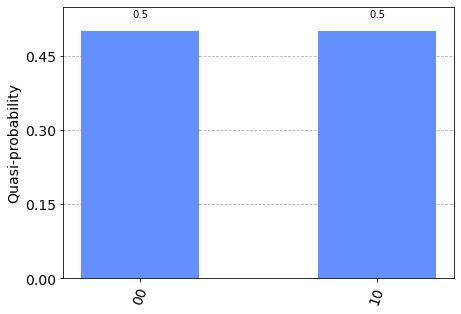
\includegraphics[]{firsthisto.png}
\end{center}
H κατάσταση που λάβαμε είναι η $\frac{\ket{00}+\ket{01}}{\sqrt{2}}$  δηλαδή άμα μετρήσουμε το πρωτο \textlatin{bit} θα είναι σίγουρα $\ket{0}$\\

Για την \textlatin{balanced} συνάρτηση έχουμε επιλέξει το \textlatin{oracle} $CNOT$ όπως φαίνεται παρακάτω
\begin{center}
    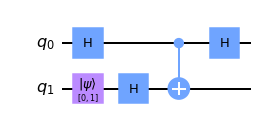
\includegraphics[]{balancedoracle.png}
    \end{center}
το αποτέλεσμα είναι
\begin{center}
    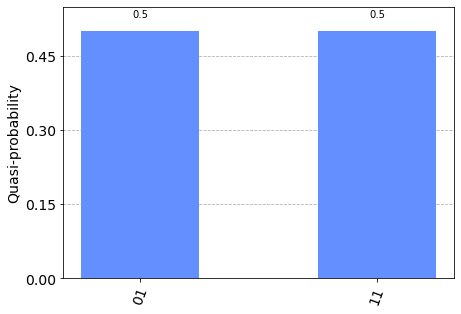
\includegraphics[]{secondhisto.png}
\end{center}
H κατάσταση που λάβαμε είναι η $\frac{\ket{10}+\ket{11}}{\sqrt{2}}$  δηλαδή άμα μετρήσουμε το πρωτο \textlatin{bit} θα είναι σίγουρα $\ket{1}$\\
\rule{\textwidth}{.5pt}

\end{document}